% -----------------------------------------------------------------------------
% Implementation
% -----------------------------------------------------------------------------
\chapter{Implementation}

As noted before the ANC system has solely been implemented in the simulation environment Matlab. The system consist of several subsystems. These subsystems will be elaborated step step and their functioning will be demonstrated.\\
The complete source code can be found in the \color{blue}\href{https://github.com/leonardberresheim/MA---Active-Noise-Control-in-Spatial-Domains/tree/main/Matlab}{projects github repository} \color{black} and is free to use, change and share without restrictions.

\section{Spherical Harmonics Decomposition}
The accuracy of the spherical harmonics decomposition in (\ref{eq:primary_noise_field}) with it's truncation degree will be demonstrated using a plane wave \textit{(see figure \ref{fig:planeWaveExp}}) as the exact harmonic coefficients can be calculated using (\ref{eq:plane_wave_coefficients})
\begin{figure}
    \centerline{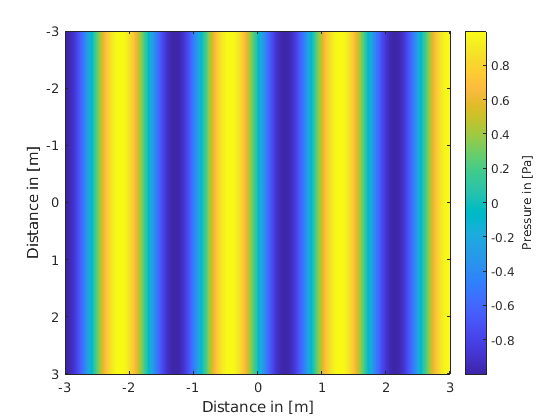
\includegraphics{LaTeX/images/plots/plane_Wave_exponent_form.png}}
    \caption{Plane wave in exponent form}
    \label{fig:planeWaveExp}
\end{figure}

\begin{figure}
    \centerline{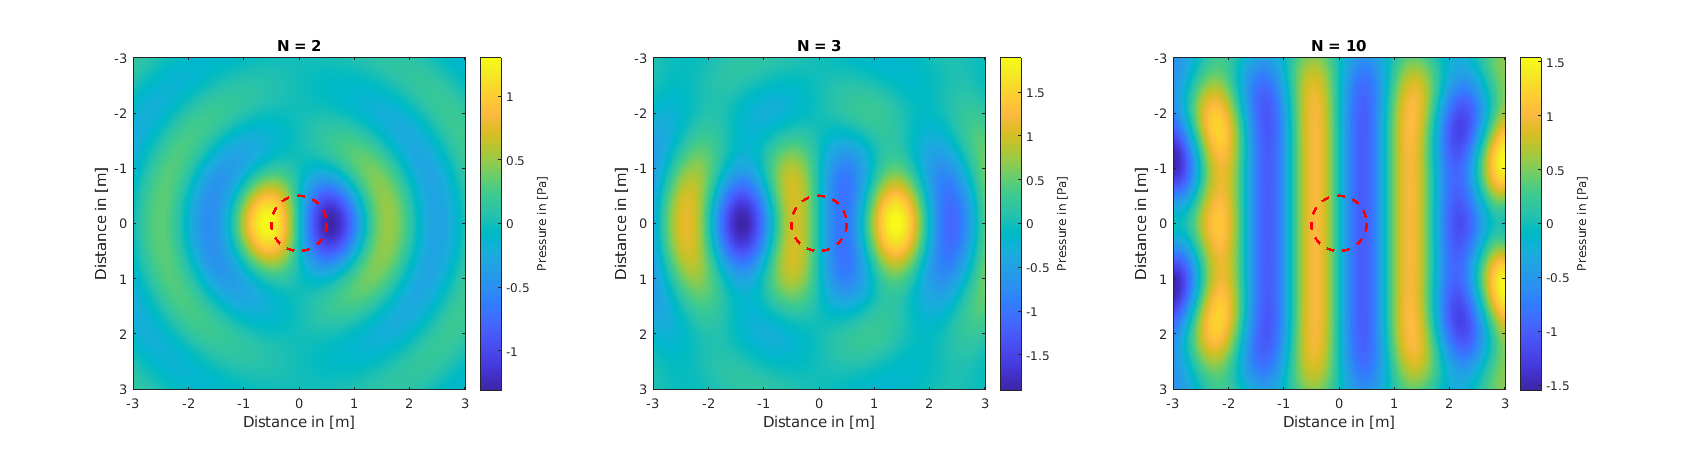
\includegraphics[width=\paperwidth]{LaTeX/images/plots/Plane_wave_harmonics_form.png}}
    \caption{Plane wave in harmonics form for number of modes 2, 3 and 10}
    \label{fig:planeWaveHarmonics}
\end{figure}
When increasing the number of modes the resulting noise field gets closer an closer to the original plane wave in figure \ref{eq:plane_wave_expansion} as can be seen in figure \ref{fig:planeWaveHarmonics}

\textit{Nota}\\
Only the imaginary part is plotted here as the behavior of the real part of the wave is analogous.